\documentclass[12pt,letterpaper]{article}
\usepackage[utf8]{inputenx} %Codificacion del texto (ISO Latin1 encoding)

\usepackage{fancyhdr} %Permite acomodar a tu gusto la parte de arriba y
% abajo del documento
\usepackage[spanish]{babel} %Permite definir el idioma del dcumento
\usepackage{graphicx} %Permite exportar imagenes en formato eps
\usepackage{caption}
\usepackage{subcaption}
\usepackage{url} %Tipo de fuente para correos y paginas
\usepackage{pgf}
\usepackage{fleqn}
\usepackage{amssymb}
\usepackage{amsmath}
\usepackage{fancyvrb}
\usepackage{makeidx}
\usepackage{colortbl} %Permite colocar colores a las tablas
\usepackage{booktabs}
\usepackage{moreverb}
\usepackage[final]{pdfpages}
%%%%%%%%%%
%Margenes%
%%%%%%%%%%
\parskip 1mm %Espacio entre parrafos

\setlength{\topmargin}{0pt}
\topmargin      0.5cm
\oddsidemargin	0.1cm  % Ancho Letter 21,59cm
\evensidemargin 0.5cm  % Alto  Letter 27,81cm
\textwidth	17cm%15.5cm
\textheight	21.0cm
\headsep	4 mm
\parindent	0.5cm
%%%%%%%%%%%%%%%%%%%%%%
%Estilo del documento%
%%%%%%%%%%%%%%%%%%%%%%
\pagestyle{fancyplain}

%%%%%%%%%%%%%%%%%%%%%%%%%%%%%%%%%%%%%%%%%%%
%Fancyheadings. Top y Bottom del documento%
%%%%%%%%%%%%%%%%%%%%%%%%%%%%%%%%%%%%%%%%%%%
% Recuerde que en este documento la portada del documento no posee
% numeracion, pero de igual manera llamaremos a esa primera pagina la numero
% 1, y la que viene la dos. Esto es para tener una idea de las que
% llamaremos pares e impares
\lhead{Investigación de Operaciones I} %Parte superior izquierda
\rhead{\bf \it Tarea 4} %Parte superior derecha
\lfoot{\it } %Parte inferior izquierda. \thepage indica
% el numero de pagina
\cfoot{} %Parte inferior central
\rfoot{\bf \thepage} %Parte inferior derecha
\renewcommand{\footrulewidth}{0.4pt} %Linea de separacion inferior

\newcommand{\primaria}[1]{
	\textbf{\underline{#1}}
}

\newcommand{\foranea}[1]{
	\textbf{\textsl{#1}}
}

\newcommand{\primyfor}[1]{
	\underline{\foranea{#1}}
}

\makeatletter
\newcommand\subsubsubsection{\@startsection {paragraph}{1}{\z@}%
                                   {-3.5ex \@plus -1ex \@minus -.2ex}%
                                   {1.5ex \@plus.2ex}%
                                   {\normalfont\bfseries}}
                       
                                
                                 
\newcommand\subsubsubsubsection{\@startsection {subparagraph}{1}{\z@}%
                                   {-3.5ex \@plus -1ex \@minus -.2ex}%
                                   {1.5ex \@plus.2ex}%
                                  
                                   {\normalfont\bfseries}}


\makeatother
 

\begin{document}
\title{Investigación de Operaciones I \\ \begin{Large}Tarea 4\end{Large}} 
\author{Victor Gonzalez (2.773.029-9)
\and Cesar Muñoz (2.973.053-0)}
\date{\today}
\maketitle

\section{Hidroeléctrica Zeus}
\subsection{Flujo máximo a los generadores}
Para determinar el flujo máximo hacia cada uno de los generadores, primero se deben identificar los distintos caminos desde el nodo 1 hacia el nodo 6.

Suponiendo que los flujos no se pueden devolver a nodos anteriores, podemos decir que se generan los siguientes caminos:

\begin{enumerate}
\item $1\to2\to5\to6$
\item $1\to2\to3\to6$
\item $1\to2\to5\to3\to6$
\item $1\to2\to3\to5\to6$
\item $1\to2\to3\to4\to6$
\item $1\to2\to5\to3\to4\to6$
\item $1\to3\to6$
\item $1\to3\to5\to6$
\item $1\to3\to2\to5\to6$
\item $1\to3\to4\to6$
\item $1\to4\to6$
\item $1\to4\to3\to6$
\item $1\to4\to3\to2\to5\to6$
\item $1\to4\to3\to5\to6$
\end{enumerate}

Ahora, tomamos algun camino conveniente para calcular los flujos. Haremos esto de manera gráfica para hacer más entendible el trabajo.

Se utilizará la notación ``$X,Y$", donde $Y$ representa el flujo acumulado en ese vértice, y $X$ la capacidad no utilizada de ese vértice.

Primero, tomaremos la ruta que comprende los nodos $1\to2\to5\to6$. Dado que el máximo flujo en ese camino es $30$, se resta esa capacidad a todos los vértices, y se agrega a todos los flujos acumulados:

\begin{figure}[htbp]
        \centering
        \begin{subfigure}[htbp]{8cm}
                \centering
                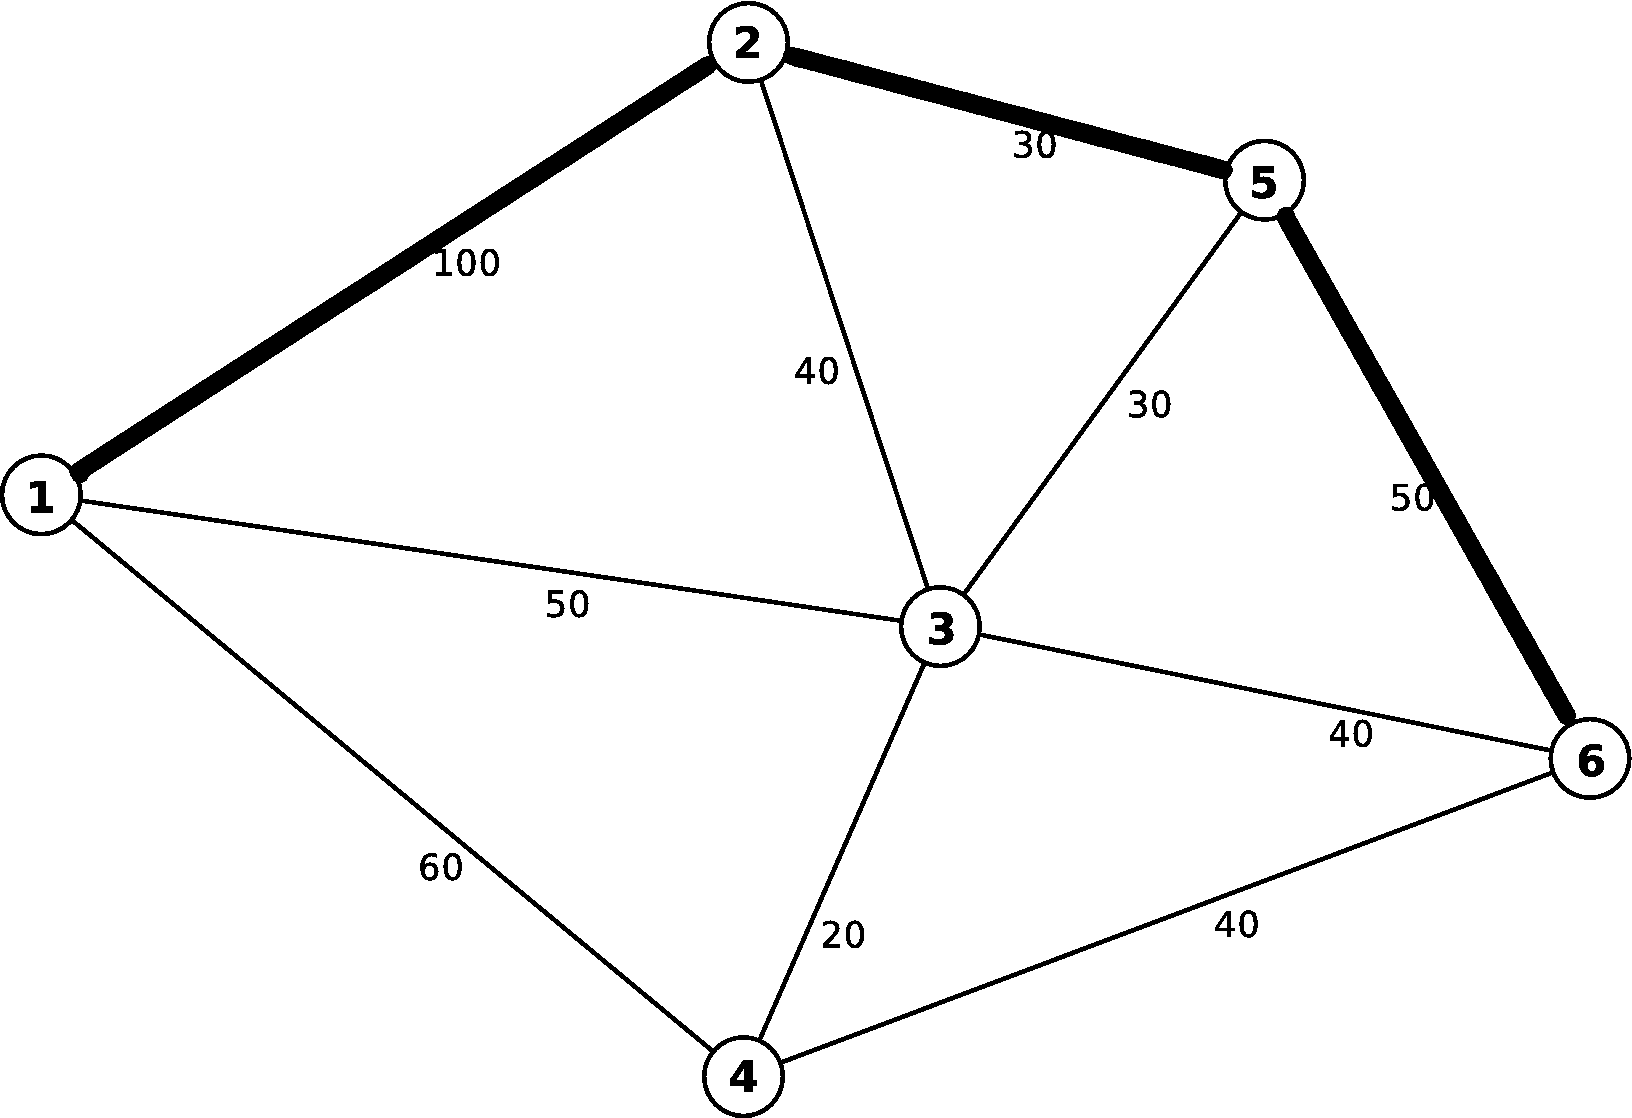
\includegraphics[width=8cm]{./it0.png}
                \caption{Camino elegido}
        \end{subfigure}
        \begin{subfigure}[htbp]{8cm}
                \centering
                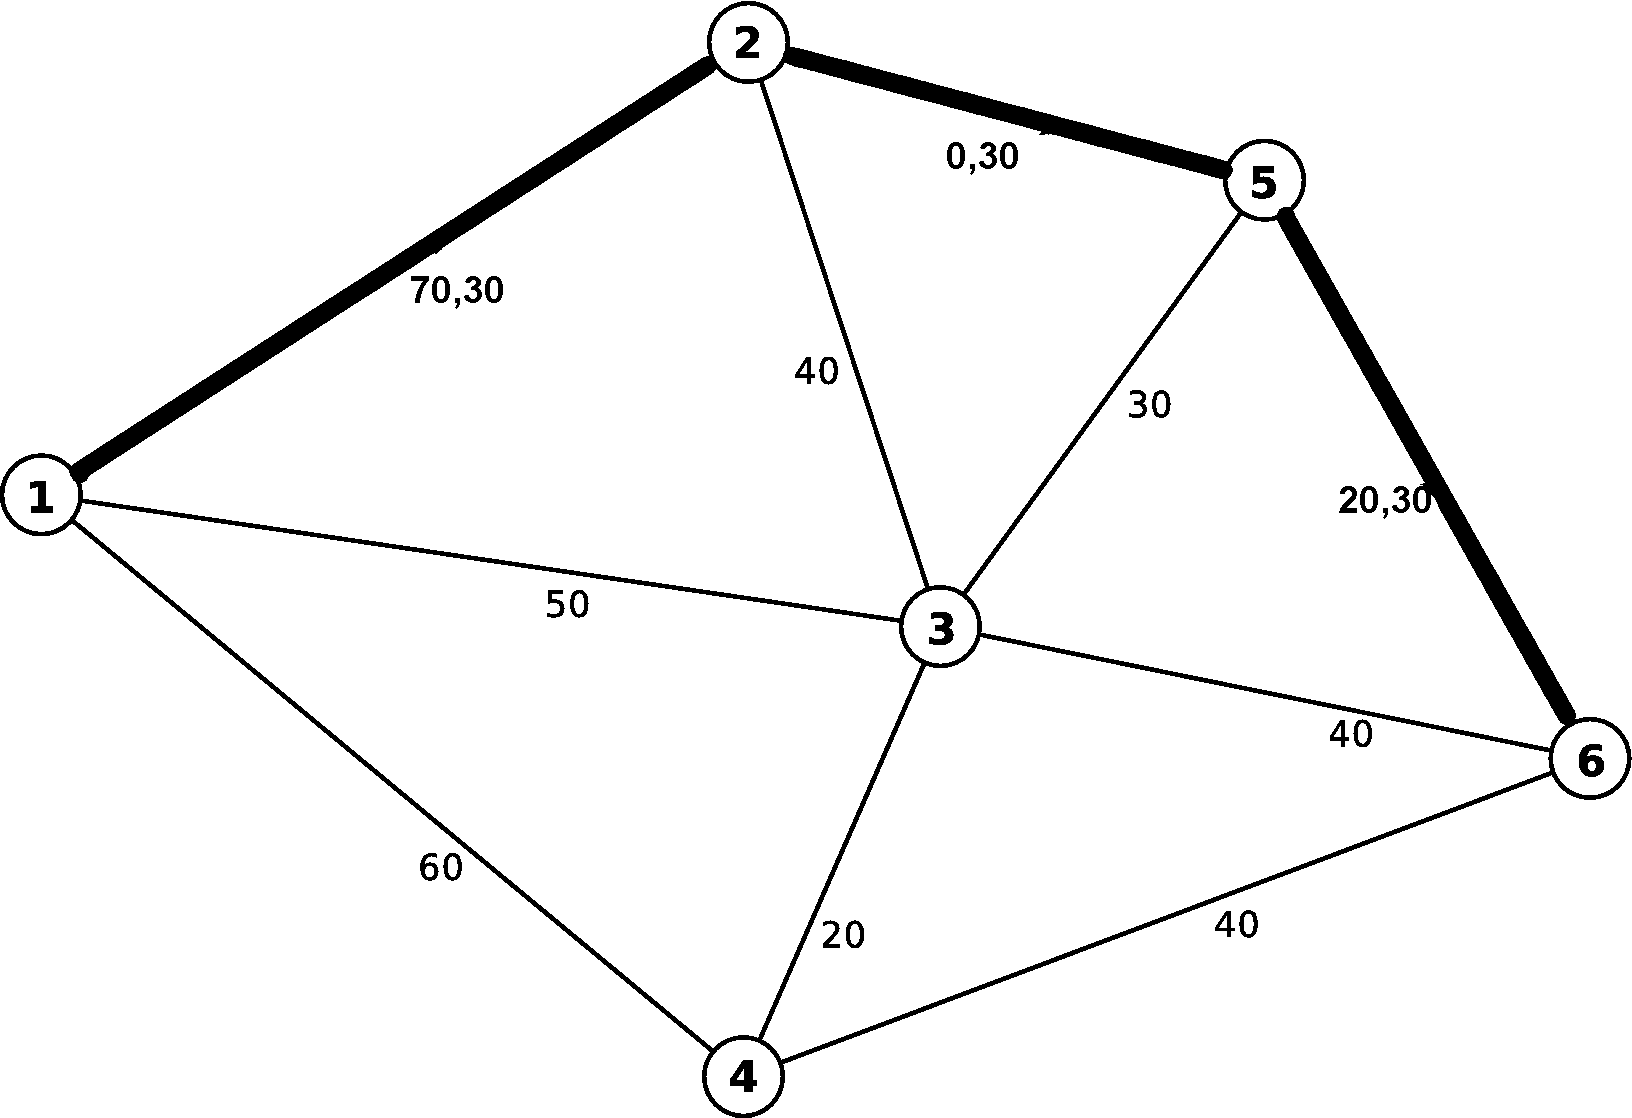
\includegraphics[width=8cm]{./it1.png}
                \caption{Camino iterado}
        \end{subfigure}
\end{figure}

De inmediato notamos que el vértice entre los nodos $2\to5$, se ha ocupado toda la capacidad, por lo que todos los caminos que utilicen ese vertice, ya no serán ``iterables". Por lo tanto, los caminos: $(1\to2\to5\to3\to6)$, $(1\to2\to5\to3\to4\to6)$, $(1\to3\to2\to5\to6)$ y $(1\to4\to3\to2\to5\to6)$, ya no se considerarán para futuras iteraciones.

Luego, elegimos el camino $1\to2\to3\to5\to6$, y aplicamos el mismo algoritmo, para todo el resto de los caminos que van quedando disponibles:

\begin{figure}[htbp]
        \begin{subfigure}[htbp]{8cm}
                \centering
                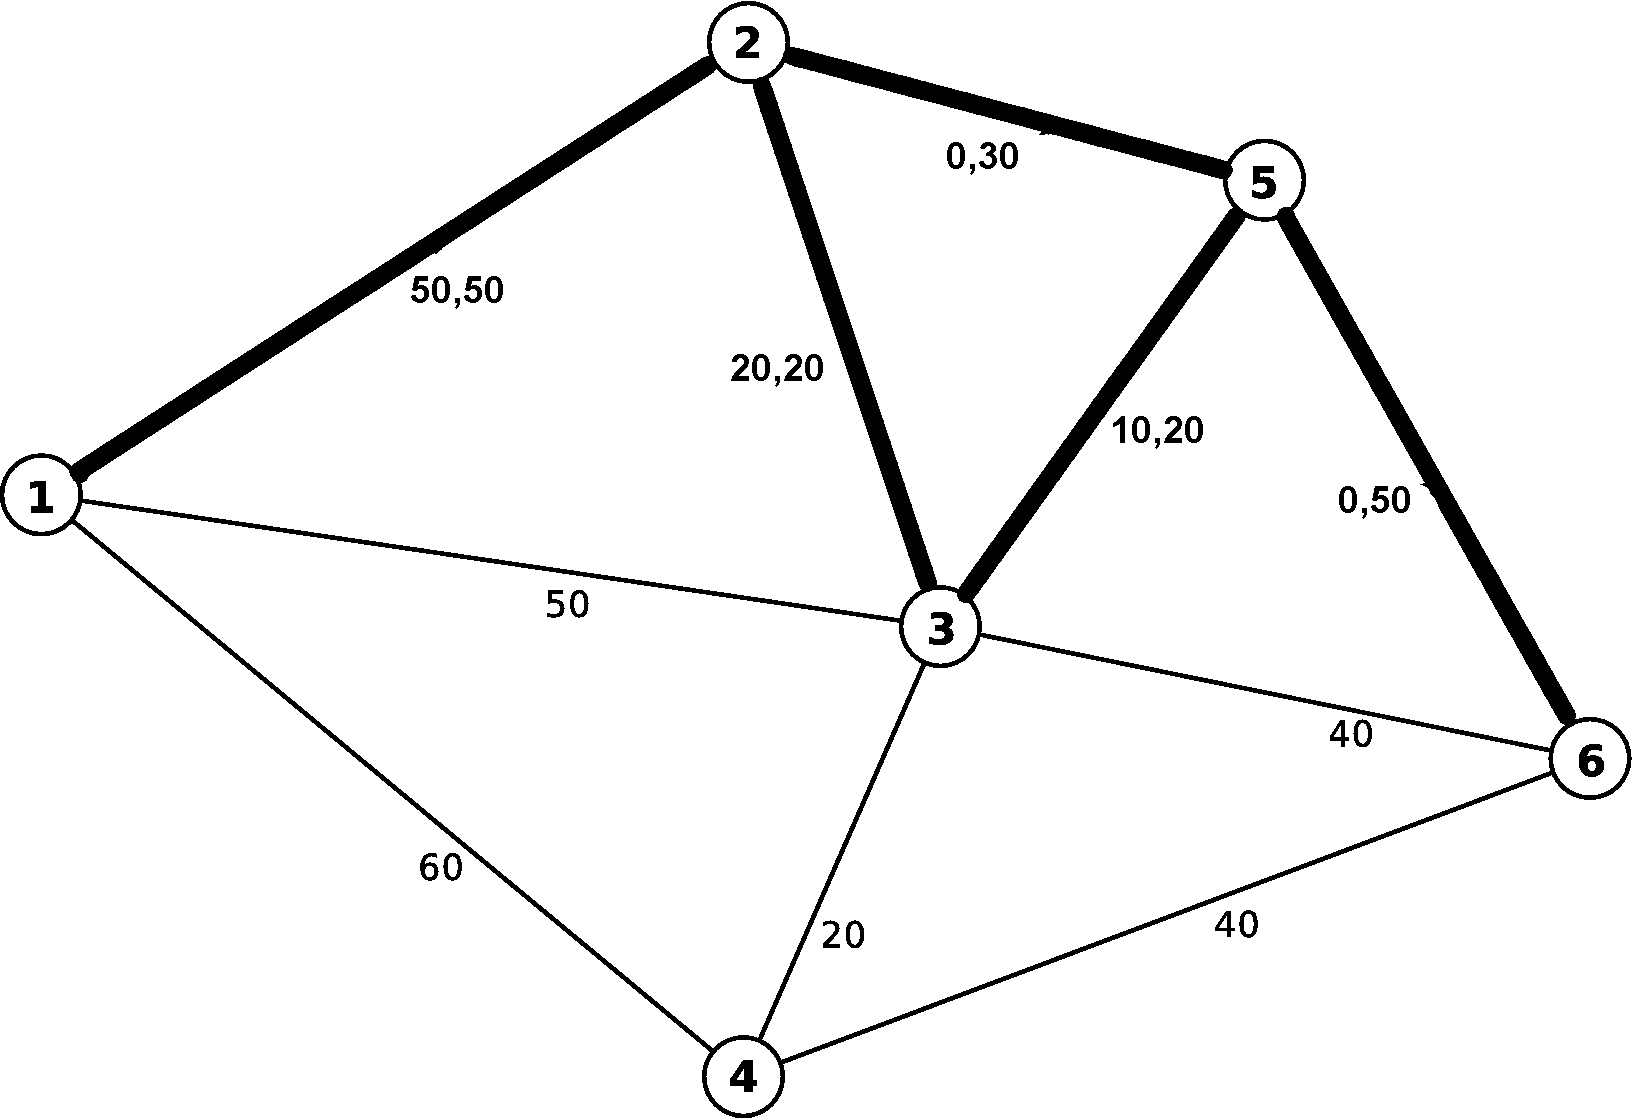
\includegraphics[width=8cm]{./it2.png}
                \caption{Camino $1\to2\to3\to5\to6$}
        \end{subfigure}
        \begin{subfigure}[htbp]{8cm}
                \centering
                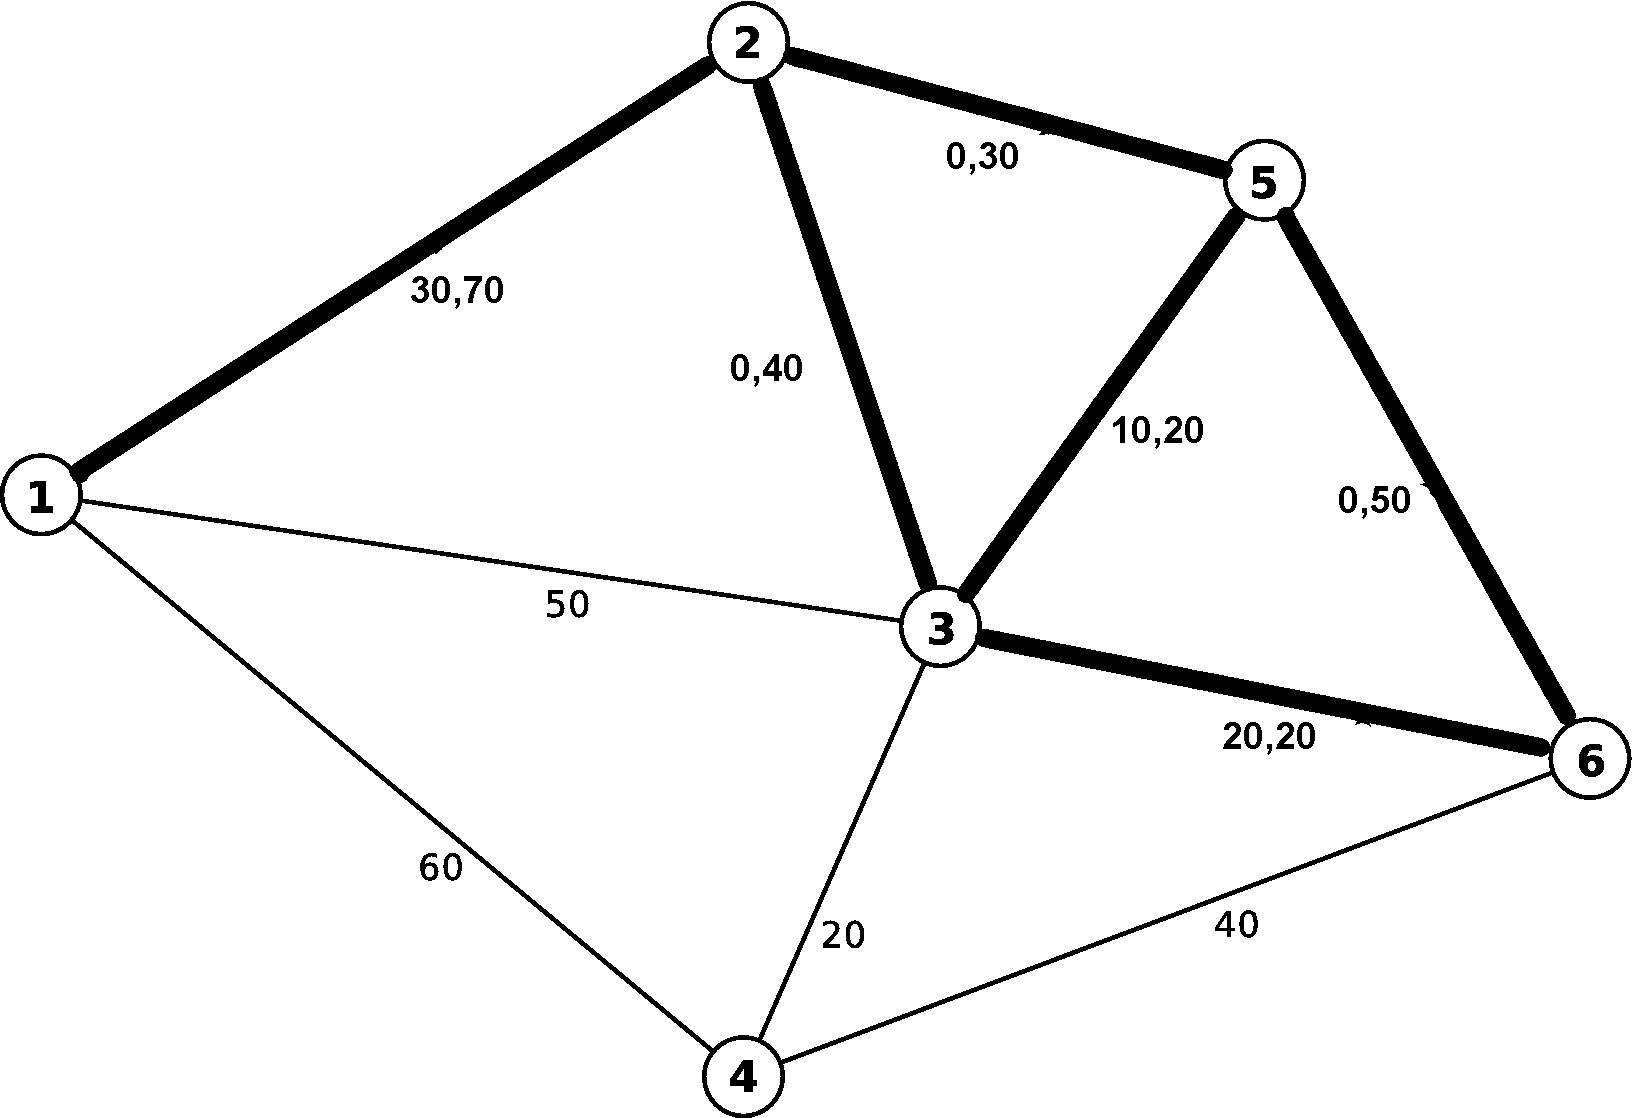
\includegraphics[width=8cm]{./it3.png}
                \caption{Camino $1\to2\to3\to6$}
        \end{subfigure}
\end{figure}

\begin{figure}[htbp]
        \begin{subfigure}[htbp]{8cm}
                \centering
                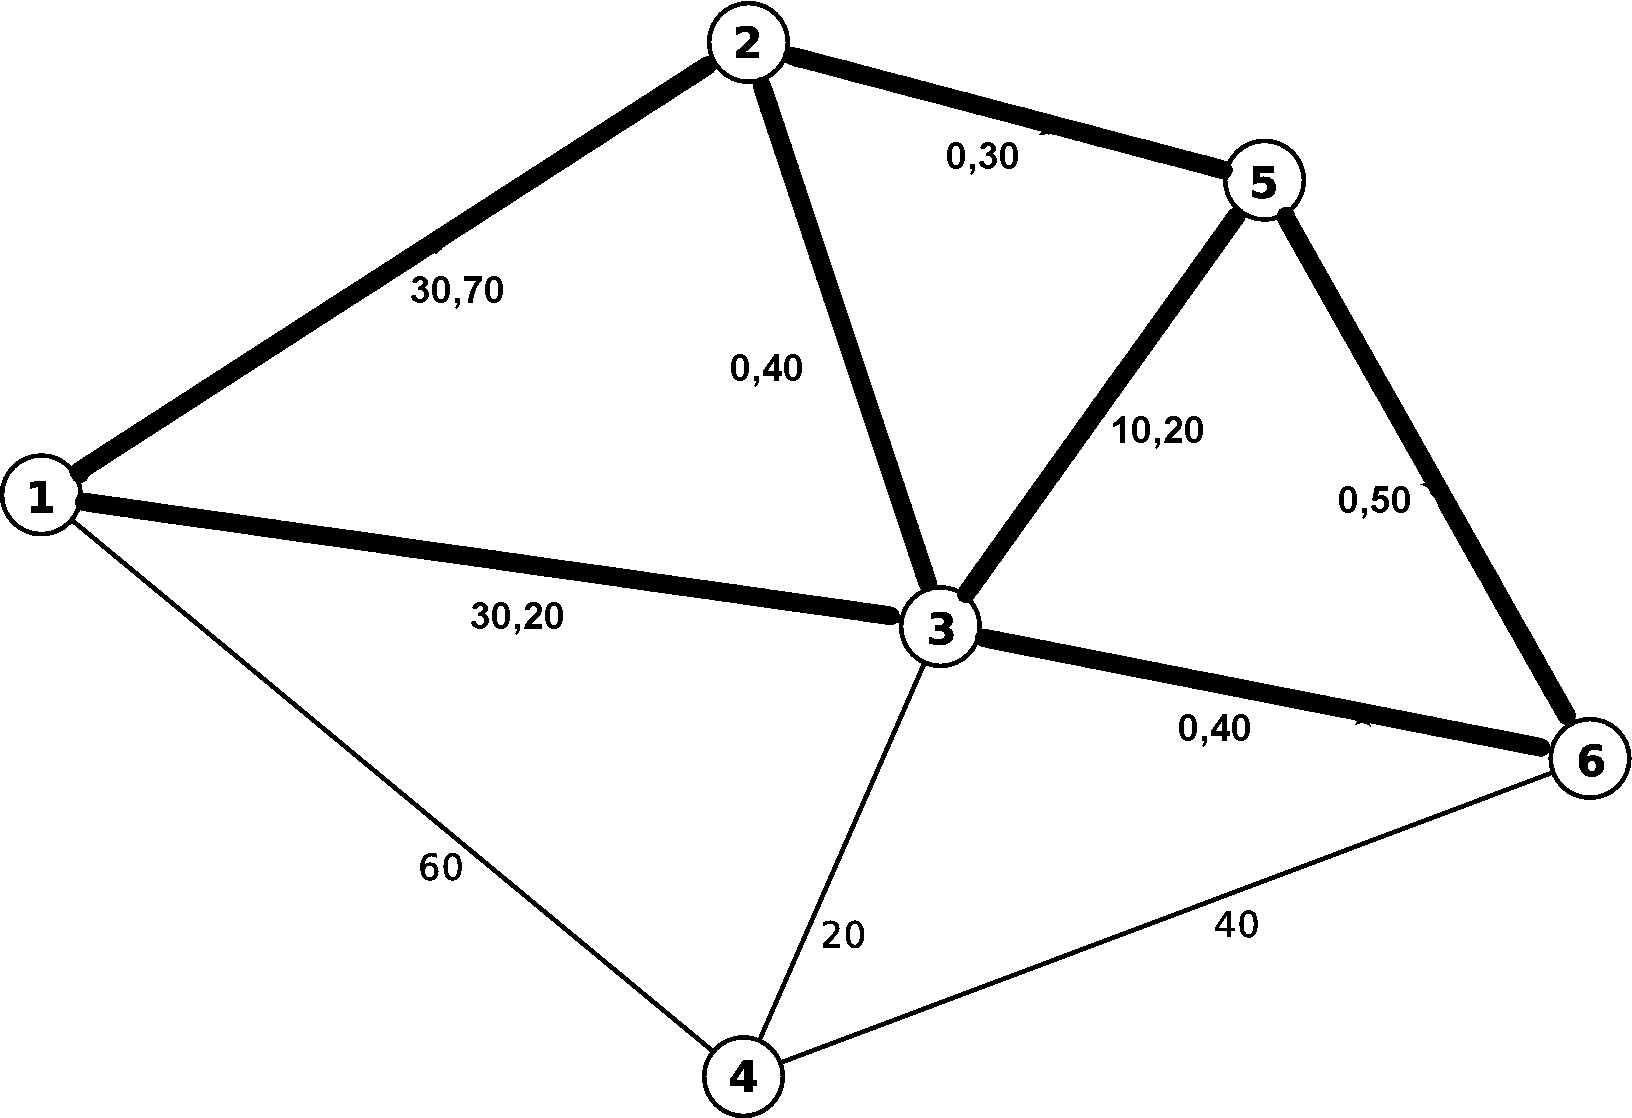
\includegraphics[width=8cm]{./it4.png}
                \caption{Camino $1\to3\to6$}
        \end{subfigure}
        \begin{subfigure}[htbp]{8cm}
                \centering
                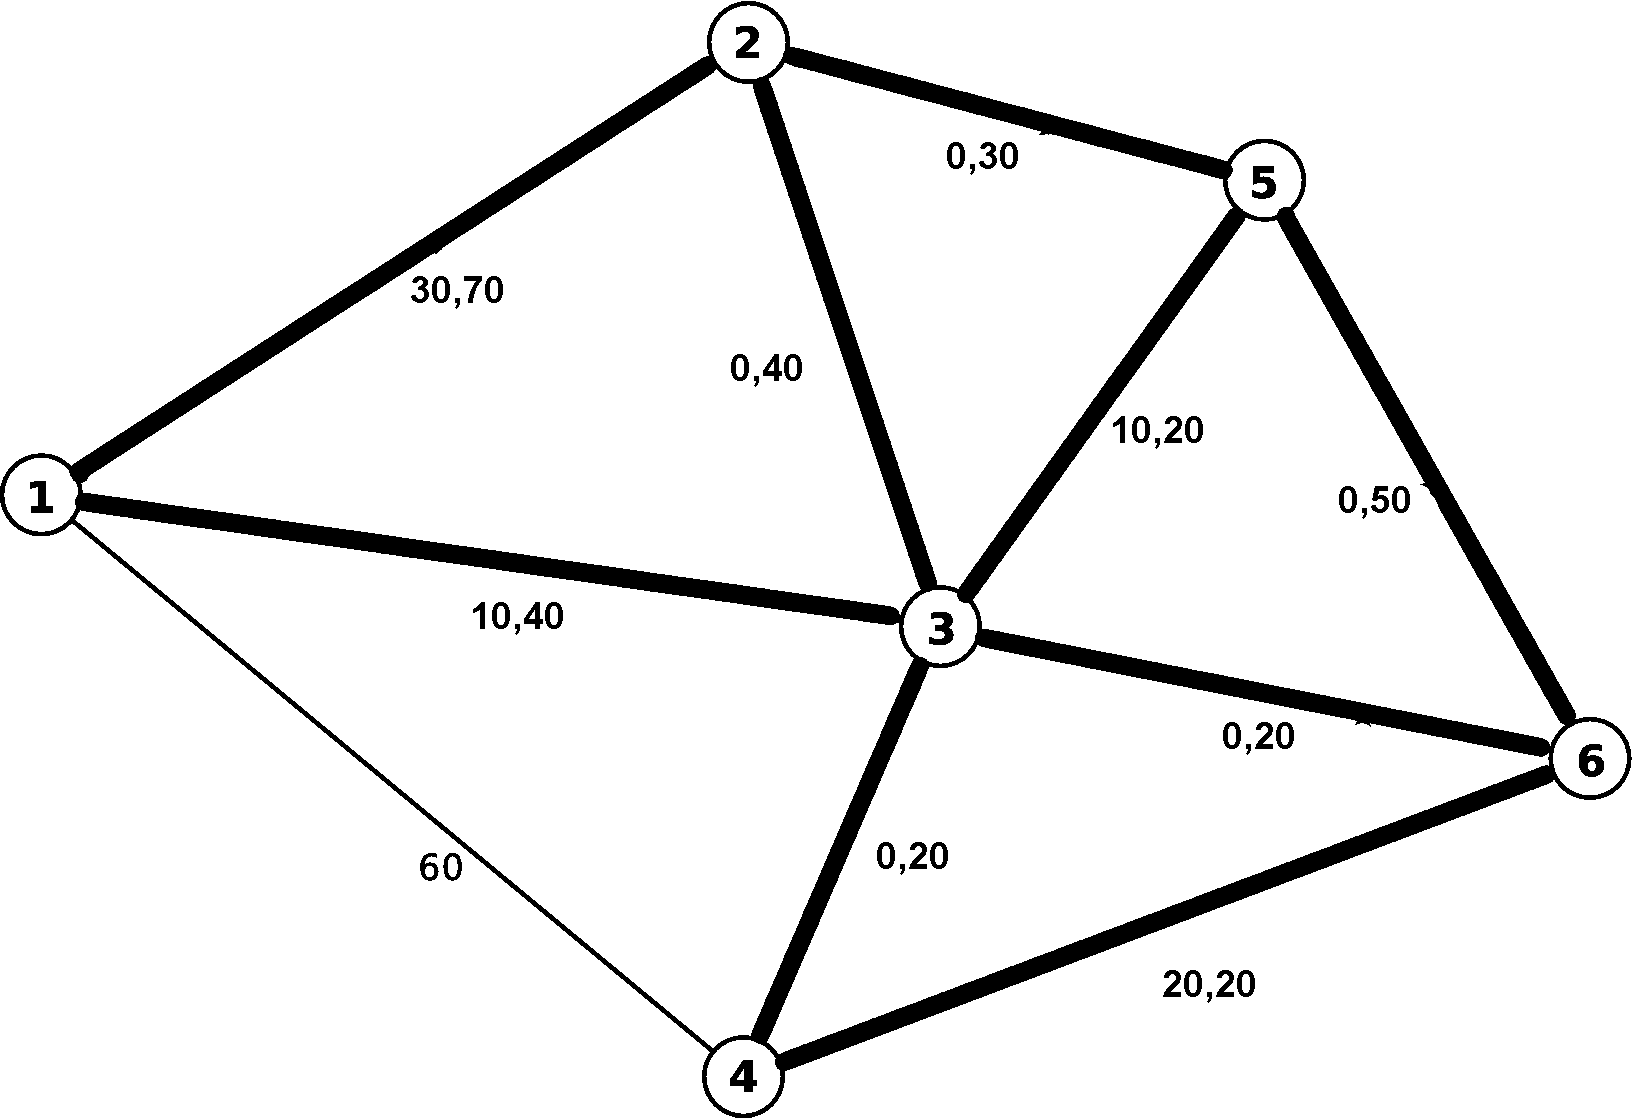
\includegraphics[width=8cm]{./it5.png}
                \caption{Camino $1\to3\to4\to6$}
        \end{subfigure}
\end{figure}

\begin{figure}[htbp]
        \begin{subfigure}[htbp]{8cm}
                \centering
                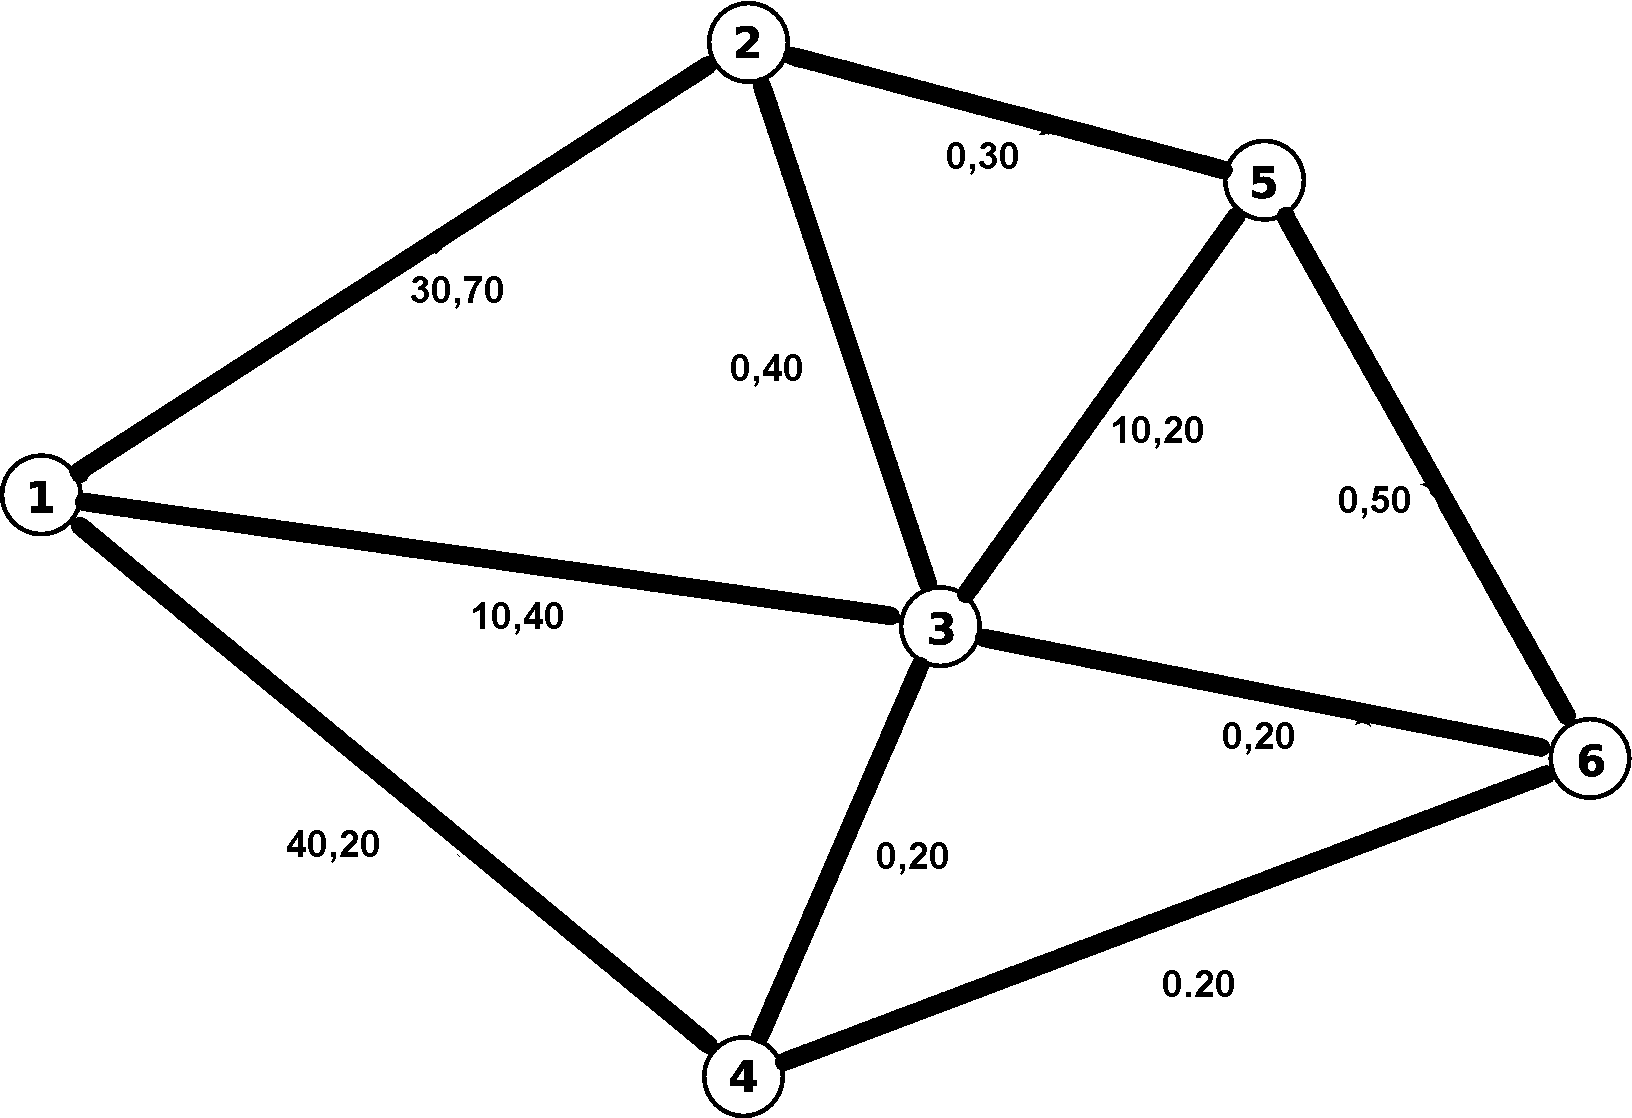
\includegraphics[width=8cm]{./it6.png}
                \caption{Camino $1\to4\to6$}
        \end{subfigure}
\end{figure}
\newpage
Luego, el grafo de flujos ya no es iterable, por lo que se ha encontrado una solución a el flujo que corre por la Hidroeléctrica Zeus.

\subsection{Modelo de programación lineal}
Existen 3 condiciones que se deben cumplir:

\begin{enumerate}
\item El flujo que entra a un nodo, es el mismo flujo que sale de ese nodo.
\item El flujo que pasa por un nodo no puede ser superior a su capacidad.
\item El flujo que sale del primer nodo debe ser igual al flujo que llega al último nodo.
\end{enumerate}

Teniendo estos elementos en consideración, se puede establecere un modelo de programación lineal, donde $X_{i,j}$ representa el flujo que pasa entre los nodos $i$ y $j$. Luego, debemos maximizar el flujo que llega al nodo final, y que sale del nodo inicial, por lo tanto, nuestra función objetivo es simplemente:
\begin{center}
$max$ $z=F$
\end{center}

Luego, para las condiciones de los nodos extremos, se puede decir lo siguiente:
\begin{center}
$X_{1,2} + X_{1,3} + X_{1,4} - F = 0$\\
$X_{5,6} + X_{3,6} + X_{4,6} -F = 0$
\end{center}

Hasta ahora tenemos las condiciones de borde y la función objetivo, por lo que hay que generar las condiciones para que los flujos que entran y salen de un nodo, sean los mismos. Para esto basta decir:
\begin{center}
$X_{1,2} + X_{3,2} - X_{2,5} - X_{2,3} = 0$\\
$X_{1,3} + X_{2,3} + X_{4,3} + X_{5,3} - X_{3,2} - X_{3,5} - X_{3,6} - X_{3,4} = 0$\\
$X_{1,4} + X_{3,4} - X_{4,3} - X_{4,6} = 0$\\
$X_{2,5} + X_{3,5} - X_{5,3} - X_{5,6} = 0$
\end{center}

Luego, solo queda definir las capacidades de cada arco, los cuales se definen de la siguiente forma:

\begin{figure}[htbp]
        \begin{subfigure}[htbp]{4cm}
                \centering
                $X_{1,2} \leq 100$\\
                $X_{1,3} \leq 50$\\
                $X_{1,4} \leq 60$\\
                $X_{2,3} \leq 40$
        \end{subfigure}
        \begin{subfigure}[htbp]{4cm}
                \centering
                $X_{3,2} \leq 40$\\
                $X_{2,5} \leq 30$\\
                $X_{3,5} \leq 30$\\
                $X_{5,3} \leq 30$
        \end{subfigure}
        \begin{subfigure}[htbp]{4cm}
                \centering
                $X_{3,4} \leq 20$\\
                $X_{4,3} \leq 20$\\
                $X_{3,6} \leq 40$\\
                $X_{4,6} \leq 40$\\
                $X_{5,6} \leq 50$
        \end{subfigure}
\end{figure}

\subsection{Programación en \textit{lp\_solve}}
El código utilizado para resolver este problema en \textit{lp\_solve}, se puede ver a continuación:

\begin{verbatim}
/* Funcion objetivo: maximizar flujo */
max F;
/* Condiciones */
/* Origen */
x12 + x13 + x14 - F = 0;
/* Destino */
x56 + x36 + x46 - F = 0;
/* Capacidades (se omiten arcos que no aportan al problema como x52) */
x12 <= 100;
x13 <= 50;
x14 <= 60;
x23 <= 40;
x32 <= 40;
x25 <= 30;
x35 <= 30;
x53 <= 30;
x34 <= 20;
x43 <= 20;
x36 <= 40;
x46 <= 40;
x56 <= 50;
/* Lo que entra a un nodo, es lo mismo que sale */
x12 + x32 - x25 - x23 = 0; /* nodo 2 */
x13 + x23 + x43 + x53 - x32 - x35 - x36 - x34 = 0; /* nodo 3 */
x14 + x34 - x43 - x46 = 0; /* nodo 4 */
x25 + x35 - x53 - x56 = 0;/* nodo 5 */
\end{verbatim}

Lo cual entrega como resultado lo siguiente:

\begin{verbatimtab}[4]
Value of objective function: 1e+30

Actual values of the variables:
max                         1e+30
F                             130
x12                            30
x13                            50
x14                            50
x56                            50
x36                            40
x46                            40
x23                             0
x32                             0
x25                            30
x35                            20
x53                             0
x34                             0
x43                            10
\end{verbatimtab}

Claramente, este no es el mismo resultado que obtuvimos previamente, pero es una de las soluciones.
\end{document}